\documentclass[hidelinks, 12pt, oneside]{article}
\usepackage{bookmark}
\usepackage{graphicx}
\usepackage{hyperref}
\usepackage{titlesec}
\setcounter{secnumdepth}{4}
\usepackage[utf8]{inputenc}
\usepackage[english]{babel}
\usepackage{color}


\begin{document}

	\begin{center}
    \centering
    
%University logo
    
\includegraphics[width=144px]{img/icon.png}
    \rule{0\linewidth}{0.15\linewidth}\par
    
    		\begin{center}
		{\uppercase{\Large User Manual\par}}
   		{\Large iCrawler \par}
   			\vspace{1cm} 
   		{\Large Emilio Mumba  \par} 
    		\vspace{1cm}
		   		
    		{\Large The 5 Concurrent Nodes \par} 
    		\vspace{1cm}
		
		{\normalsize Khathutshelo Shaun Matidza\par}
		{\normalsize Sylvester Sandile Mpangane\par}
		{\normalsize Thabang Michael Letageng\par}
		{\normalsize Matthew Nel\par}
		
		\end{center}

		\textbf{}		
		\centering
		\vspace{2cm}
		Department of Computer Science, University of Pretoria

		
	 	{\Large  September 2015}
\end{center}
\clearpage


	\tableofcontents
	\newpage
	
	\section{Overview}
	\emph{iCrawler} is a mobile device monitoring app available for Android only. The objective of the app is to display and assist in understanding the activities performed by a mobile user as well as shedding more light into the behaviour of the mobile user. The mobile monitoring application generates reports giving the investigator quick and comprehensive data/logs. The app
uses the device's internet connection to send the data logs collected from the device to a desktop-dashboard for review. The app is absolutely free to download.\newline\newline
	 
	 \uppercase{Why use the \MakeLowercase iCrawler App:}\newline
	 \begin{itemize}
		\item Child monitoring\newline
		\emph{iCrawler} can be used by parents/guardians to monitor activities that their minor
		 children get up to.	
		\item Employee monitoring\newline
		Companies that hand out mobile devices to their employees can use the \emph{iCrawler} app to monitor any 
		unauthorized activities that employees might be getting up to.
	\end{itemize}
	\newpage
	
	
	\section{Configuration}
	
	\begin{tabular}{ |l|l| }  \multicolumn{2}{|c|}{
\includegraphics[width=0.1 \textwidth]{img/icon.png}iCrawler}
	 \\ \hline\noalign{\smallskip} \textbf{Stable release} & 1.0
	  \\\\ \noalign{\smallskip} \textbf{Development status}& Active
	  \\\\ \noalign{\smallskip}\textbf{Operating System}& Android 4.2+
	  \\\\ \noalign{\smallskip}\textbf{Platform}& Android
	  \\\\ \noalign{\smallskip}\textbf{Internet connection} & Yes
	  \\\\ \noalign{\smallskip}\textbf{Available in} & English
	  \\\\ \noalign{\smallskip}\textbf{Type}& Monitoring Application
	  \\\\ \noalign{\smallskip}\textbf{License}& Free
	  \\\\ \noalign{\smallskip}\textbf{Website}& www.github.com/u11241617/COS301-Mobile-Monitoring-App
	  %\hline
	 \end{tabular}\newpage
	%%%%%%%%%%%%%%%%%%%%%%%%%%%%%%%%%%%%%%%%%%%%%%%%%%%%%%%%%%%%%%%%%%%%%%%%%%%%%%%%%%%
	\section{User Access Levels}
		Our Github repository is private, only invited users can download the appliaction, additionaly a user has  to be registered on iCrawler to be able to have the app submit their user activities onto the dashboard, and to be able to log onto the dashboard.\newline
	\section{Installation}
	The iCrawler APK (Android Application Kit) is currently only available for download on our GitHub repository. Follow this link inorder 
	to start the download\dots\newline
		\href{url}{https://github.com/u11241617/COS301-Mobile-Monitoring-App/tree/master\\/Android\%20Project/}\\
		\emph{NB:} Open the \emph{app-release} folder to find the apk \newline \newline
		When the download has successfully completed the installation should automatically start, if not follow the following steps:\newline
	  
	 \begin{enumerate}
 	 	\item Navigate to 'File Management' from the options menu on your device
 	 	\item Under 'Device Storage', locate a folder named 'Download'
 	 	\item Locate and launch a file named 'iCrawler.apk' within this folder
 	 	\item When a 'Install blocked' popup appears, select the 'Settings' option
 	 	\item Scroll down and check the option 'Unknown Sources'
 	 	\item Another popup will appear, simply click 'OK' then 'Next' followed by 'Install'
 	 	\item On completion you will see the options 'Done' and 'Open', click 'Open' to start the app \ldots
 	\end{enumerate}\newpage


	\section{Getting Started}
	After successful installation, locate the iCrawler app icon and click on it to launch the app.
	 \begin{figure}[h!]
	 	 \caption{Launching iCrawler app}
	 	 \centering 																																	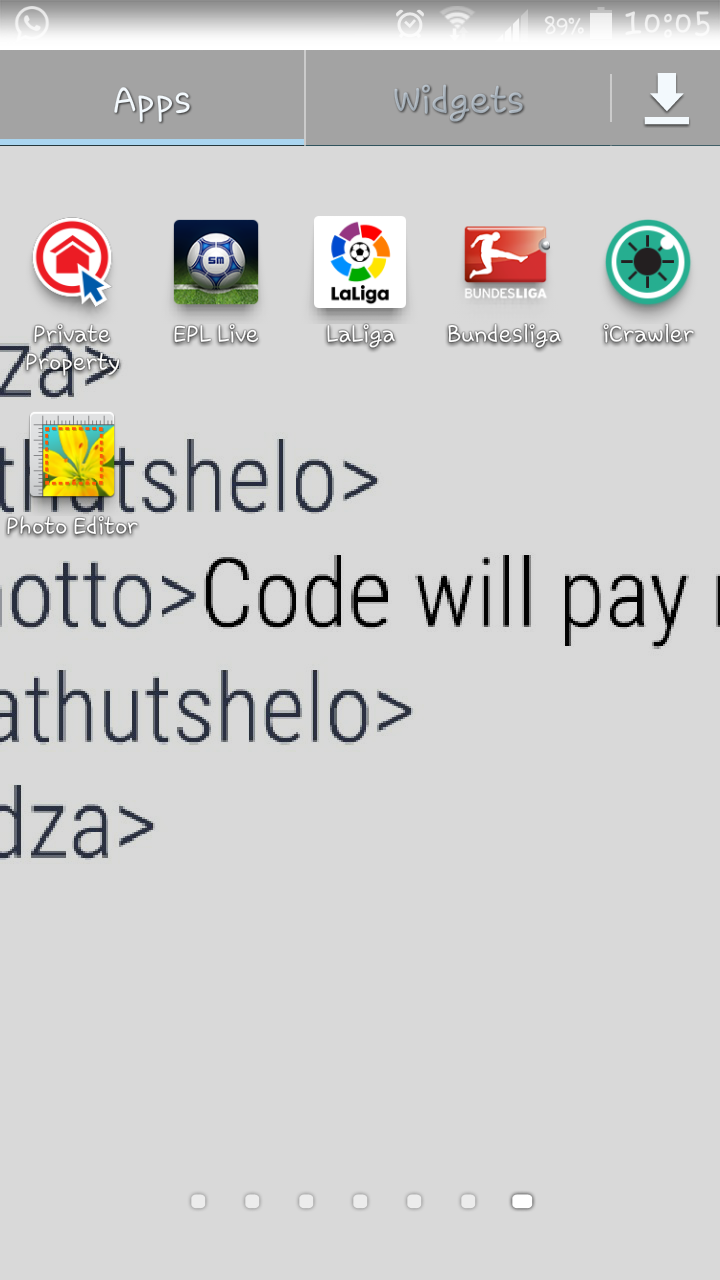
\includegraphics[width=0.5 \textwidth]{img/newImgs/appLaunch.png}
	 \end{figure}\newpage
	 
	 \begin{itemize}
	 	\item \textbf{Welcome to iCrawler}\newline
	 	This is the landing page when you launch the app. This page introduces what the app is about and also provides you
	 	with the options to either proceed with the app tour or skip to sign up/sign in.
	 	 
	 	 %Welcome page%
	 	 \begin{figure}[h!]
	 	 	\caption{Welcome to iCrawler}
	 	 	\centering 																																		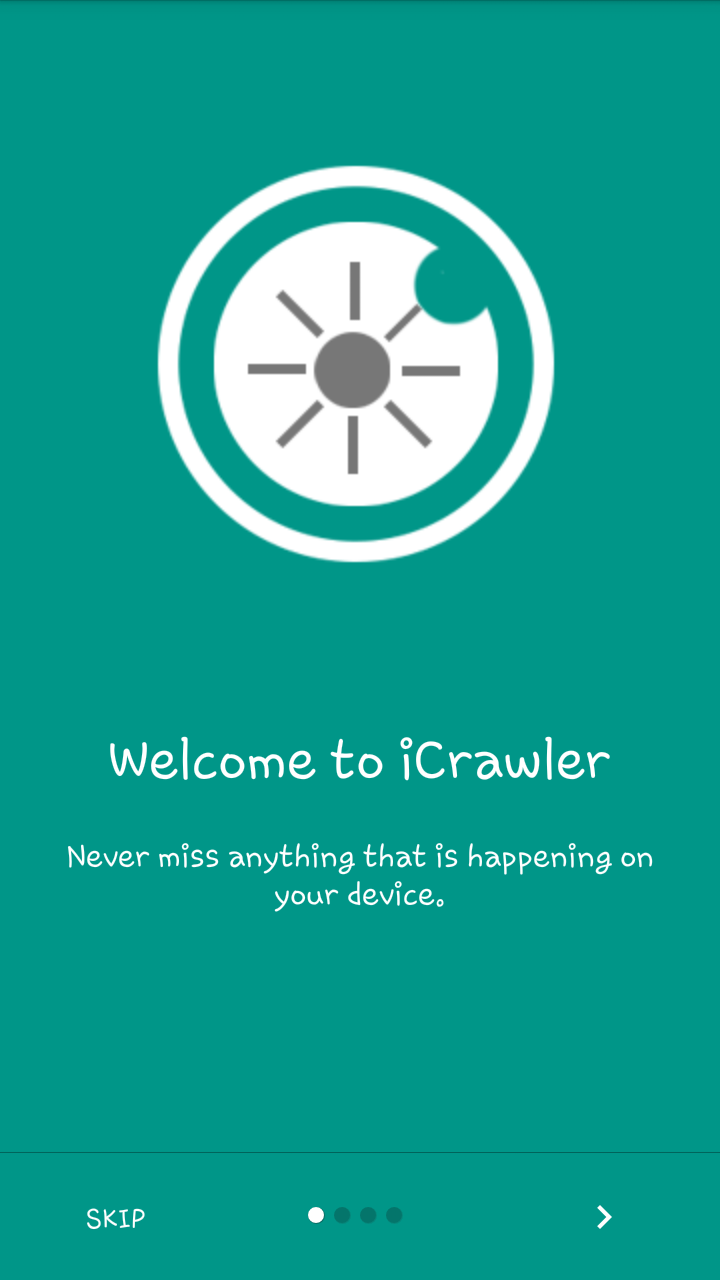
\includegraphics[width=0.5 \textwidth]{img/newImgs/landingPage.png}
	 	 \end{figure}\newpage
	 	 
		\item \textbf{Take tour}\newline
	 	If you opt to take a tour, this tour will explain all the features that come with this app.\newline\newline
	 	The app runs on the background collecting and compiling data logs of activities on your device. 
	 	 
	 	 %tourpage one%
	 	 \begin{figure}[h!]
	 	 	\caption{Never left alone}
	 	 	\centering 																																		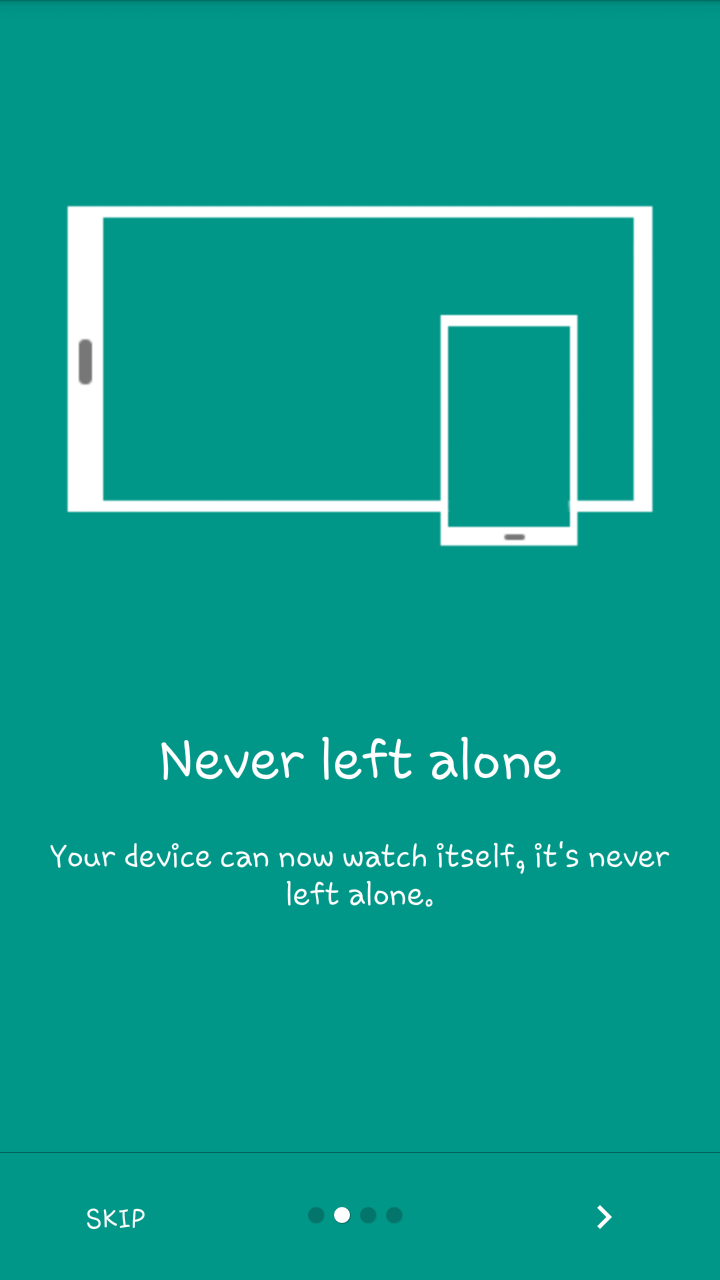
\includegraphics[width=0.5 \textwidth]{img/newImgs/tourOne.png}
	 	 \end{figure}\newpage	
	 	 
	 	 To view the compiled logs you simply log onto the web application, using either your laptop or desktop, with your credentials and 
	 	 view the collected data. 
	 	 %tourpage two%
	 	 \begin{figure}[h!]
	 	 	\caption{View monitored logs}
	 	 	\centering 																																		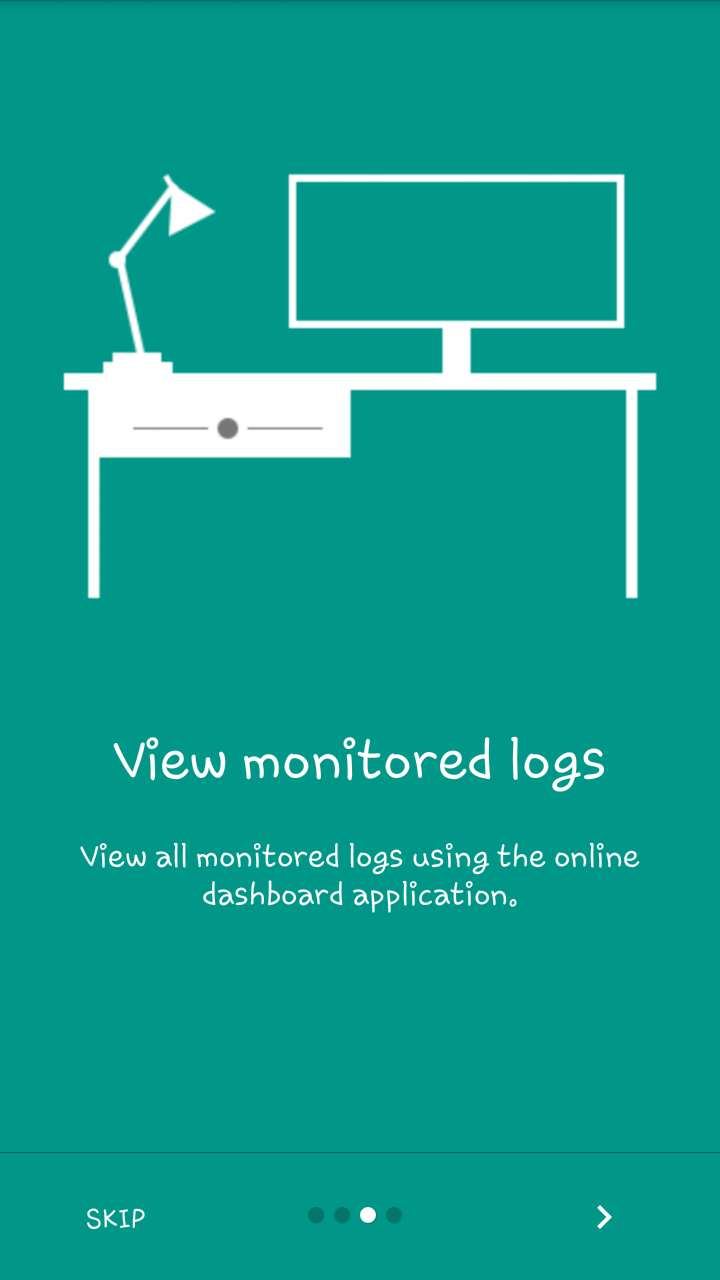
\includegraphics[width=0.5 \textwidth]{img/newImgs/tourTwo.png}
	 	 \end{figure}\newpage	 	 
	 	 
	 	 To be able to use the awesome features that come with this app, all you have to do is sign up, if you are a new user, or simply
	 	 just sign in and you are ready to go! 
	 	 %tourpage three%
	 	 \begin{figure}[h!]
	 	 	\caption{All you have to do}
	 	 	\centering 																																		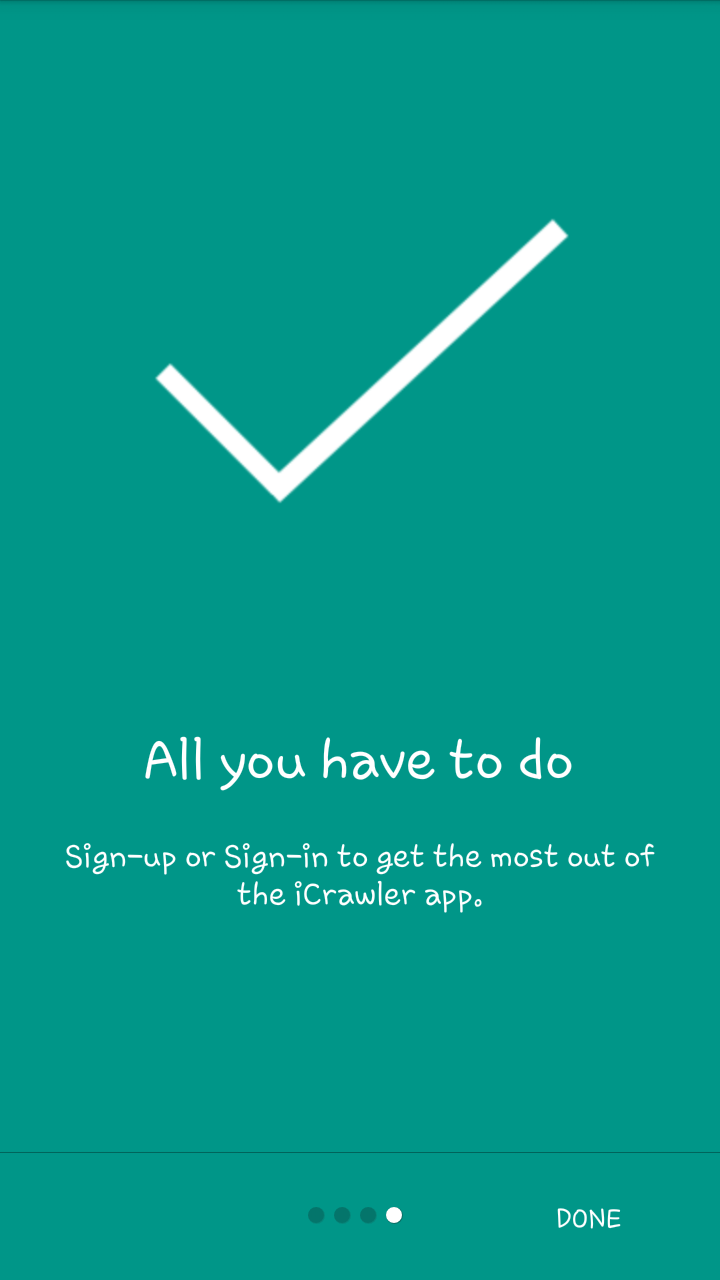
\includegraphics[width=0.5 \textwidth]{img/newImgs/tourThree.png}
	 	 \end{figure}\newpage	 	 
	 	 
	 	\item \textbf{Skip tour}\newline
	 	If you decided to skip the app tour then you get the options to Sign up or Sign in; you can still take the tour by clicking the 
	 	'Take Tour' link at the bottom.\newline
	 	By signing up or signing in, you agree to our Terms and Privacy Policy. 
	 	 
	 	 %sign up%
	 	 \begin{figure}[h!]
	 	 	\caption{Signing up}
	 	 	\centering 																																		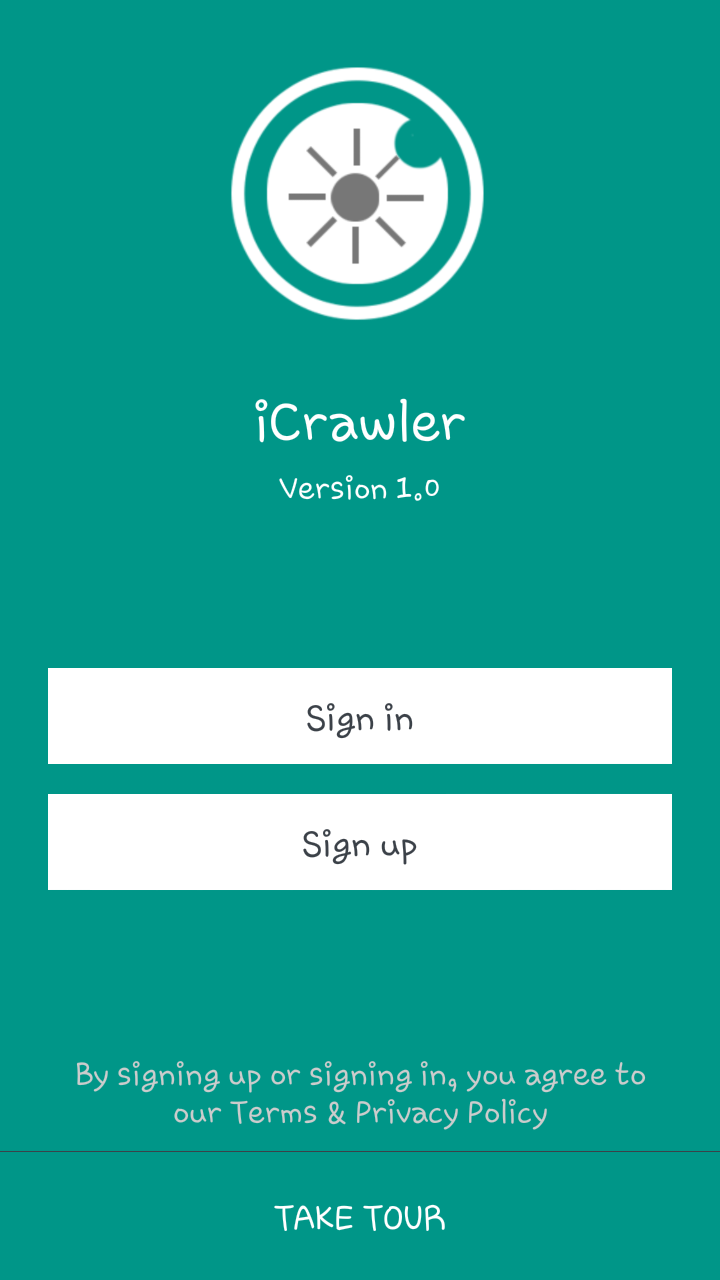
\includegraphics[width=0.5 \textwidth]{img/newImgs/homePage.png}
	 	 \end{figure}\newpage
	 	 
	 	 If you have never used the iCrawler app before, you need to sign up; simply enter your valid email address and password then
	 	click the 'orange arrow' pointing to the right in order to subscribe as a new user.
	 	
		%sign up%
	 	 \begin{figure}[h!]
	 	 	\caption{Signing up}
	 	 	\centering 																																		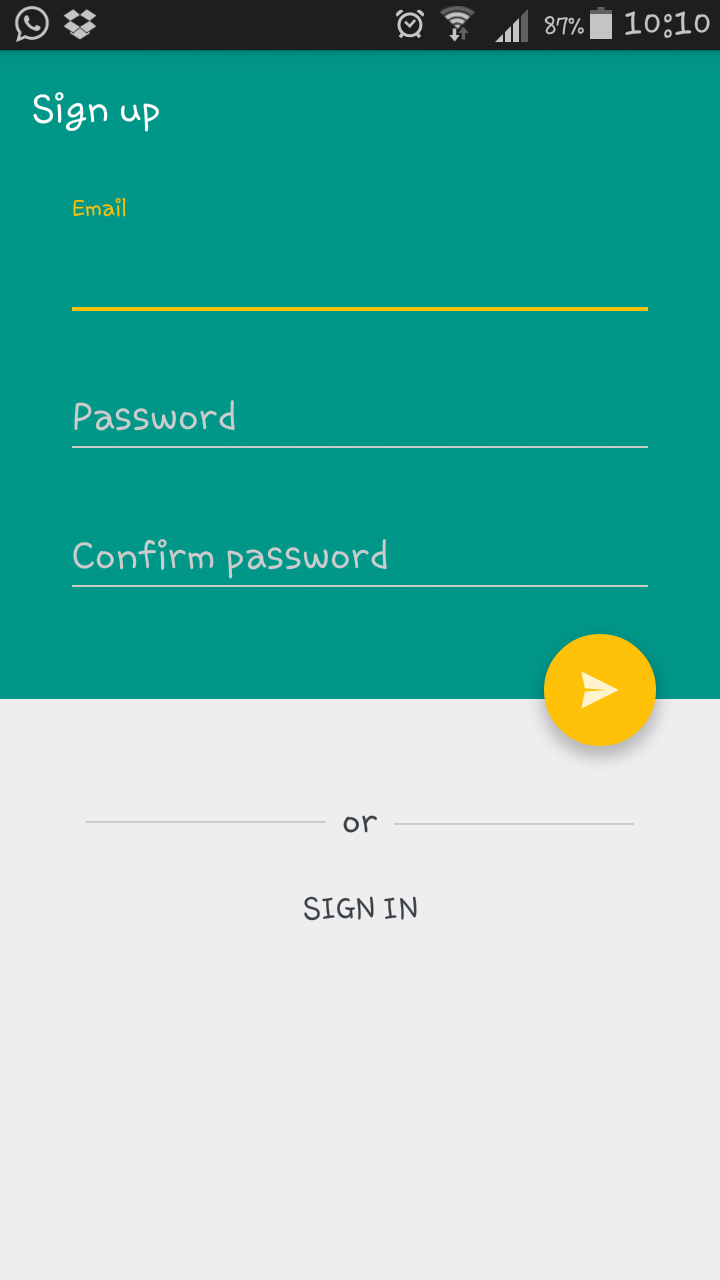
\includegraphics[width=0.5 \textwidth]{img/newImgs/signUp.png}
	 	 \end{figure}\newpage	 	 
	 	 
	 	If you have used the iCrawler app before, you need not to sign up again, simply enter your credentials and then
	 	click the 'orange arrow' pointing to the right in order to subscribe the new device. If not, click 'Sign up' to register as a new user.
	 	
	 	%sign in%
	 	 \begin{figure}[h!]
	 	 	\caption{Signing in}
	 	 	\centering 																																		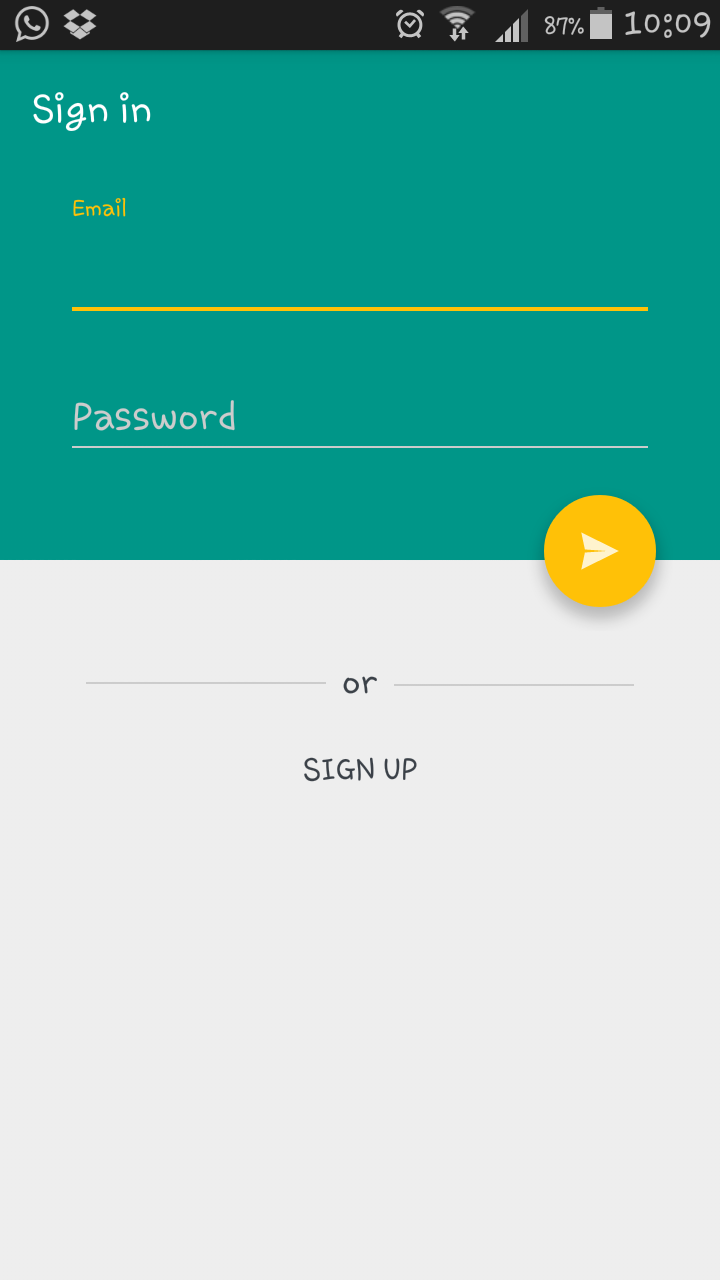
\includegraphics[width=0.5 \textwidth]{img/newImgs/signIn.png}
	 	 \end{figure}
	 	 
	 \end{itemize}\newpage
	 
	 
	\section{Using the App}
	The app runs in the background after 'Signing up or Signing in'; there is no other form of interaction with 
	the app thereafter. You can access the log reports generated via the dashboard.
	\newline\newline
	
	\section{Troubleshooting}
	The following section lists some of the iCrawler app's possible issues and resolutions:
	
	\begin{itemize}
		\item \textbf{Does not launch.} Restart your phone and try to launch the application again.
		\item\textbf{Crashes immediately after launch.} Ensure that your device meets the minimum specifications to run
		 iCrawler (See configurations). Go to Settings $\rightarrow$ Apps $\rightarrow$ Manage Apps $\rightarrow$ Running, to check if your apps are not using up all
		  your memory. Try to end all processes you do not need and re-start your phone.
		\item \textbf{Other unknown causes.} If problems continue, delete the app completely and then reinstall it.\
	\end{itemize}
		
\end{document}
